\section{Methodology}

\subsection{Research Hypothesis}
\label{sec:hypo}

For this study the main hypotheses were formulated as follows:

\begin{align*}
H_{0}&: 
\begin{minipage}[t]{0.8\linewidth}
There is no statistically significant dynamic relationship between
\gls{SMU} (PM-table) and \gls{RAPL} measurements for the
selected power domains; any observed similarity
is due to random variation.
\end{minipage}\\[0.8em]
H_{1}&:
\begin{minipage}[t]{0.8\linewidth}
\gls{SMU} (PM-table) and \gls{RAPL} measurements for the same domains
exhibit significant temporal correlation and similar trends.
\end{minipage}
\end{align*}

To test the above this work next employs:
\begin{itemize}
  \item Pearson correlation and cross-correlation test to assess dynamic
        similarity and possible time lags.
  \item Visual inspection of primary data plots to compare long-term trends
        and identify anomalies, short-term fluctuations and/or outliers.
  \item Bland–Altman plots and error metrics to describe the spread of
        differences and practical agreement.
\end{itemize}

\subsection{Test System Setup}

\subsubsection{Hardware}

All experimental data in this study was collected on a system equipped with an
AMD Ryzen 5 3600 processor, featuring six physical cores and twelve hardware
threads. The processor operated on a Gigabyte A320M-H-CF mainboard, running
\gls{BIOS} version F53, release date: January 2021.

For reproducibility, the complete hardware and software specifications of the
test environment are provided in \cref{app:hwspec}. This includes detailed
\gls{CPU}, memory, storage, \gls{GPU}, and firmware information, as well as
the software stack and driver versions used during the experiments.

\subsubsection{Software Environment}

The experiments were conducted on an up-to-date Arch Linux (rolling release)
installation with Linux kernel version 6.16.4-arch1-1.

Additional details on the compiler tool-chain, installed kernel headers, and
device drivers are provided in \cref{app:swspec}.

\subsection{Supporting Documentation}

In addition to research articles, several forms of supporting
documentation were instrumental in the preparation and execution of
this study. These resources provided both the practical foundation for
system configuration and the technical background required for working
with AMD-specific interfaces, Linux monitoring tools and kernel drivers.

The Red Hat \footcite{RedHat_Docs} documentation and ArchWiki \footcite{ArchWiki}
were frequently consulted during system setup and software preparation. These
resources were essential in the identification and configuration of key tools,
including hardware monitoring utilities, processor and/or mainboard topology
inspection tools, kernel modules and drivers, process management mechanisms, etc.
Beyond initial configuration, both sources served as references for
troubleshooting and verification of software and hardware functionality for
test system, thereby contributing directly to the reliability of the
experimental environment and setup.

For AMD-specific mechanisms, official vendor documentation proved less
useful due to it's limited accessibility and fragmented nature. In practice,
one the most valuable reference was the open-source \texttt{ryzen\_smu} kernel
driver repository \footcite{RyzenSMU_GitHub}. Alongside with the source code
it contains documentation in its accompanying README. To overcome some
challenges during methodology development the \texttt{ryzen\_monitor} repository
\footcite{RyzenMonitor_GitHub} was also used as a source of implementation and
usage (programmatic) examples of the driver. Direct inspection of mentioned
materials provided critical insights into available usage variants, functions,
\gls{PM} tables' mappings, and constraints, which were essential for the
implementation of the necessary but missing software parts required for
successful completions of this research.

A complementary source of technical insight is the informal GitHub
repository \\\emph{plops/ryzen\_managment\_linux}
\footcite{ryzen_managment_linux}, which provides annotated
explanations of the low-level behavior of the \texttt{ryzen\_smu} driver
interface. In particular, the author highlights that the \gls{SMU} driver is
\emph{on-demand} rather than polling, and implements an internal throttling
mechanism—limiting \gls{SMU} refreshes to at most 1 kHz, even if user-space
attempts to poll faster . While this project is not a formal documentation,
it helps to understand practical limitations of the \gls{PM} Table interface
and guides decisions about sampling frequency and overhead optimization
during plug-in implementation.

Intel’s official developer manuals \footcite{Intel_SDM}, which are widely
regarded as a reference standard in terms of accessibility and comprehensiveness,
were used primarily as a comparative benchmark. Their structured presentation
of hardware interfaces and architectural features highlighted the relative
scarcity and incompletion of AMD-specific documentation.

The combined use of above-mentioned sources contributes to several points of
this work:
\begin{itemize}
    \item Correct identification of measurement power domains.
    \item Reproducible platform configuration.
    \item Selection of implementation approaches for the \gls{SMU}-to-energy
        conversion.
    \item Principled discussion of the limitations and security considerations.
\end{itemize}

\subsection{Limitations and Considerations}
\label{sec:limncons}

Several limitations should be acknowledged regarding the measurement setup
and methodology.

First, the \gls{RAPL} interface on Intel-compatible \gls{CPU}s enforces a hardware
constraint on the update frequency of energy counters. Independent of how
often the counters are read, their effective resolution is limited to about
1~kHz. This design choice has been discussed in the context of limiting the
risk of side-channel attacks exploiting high-resolution power traces
\parencite{IntelRAPL, PwrLeak_2023}.

The statement in \texttt{ryzen\_managment\_linux} repository
\footcite{ryzen_managment_linux} also describes similar limitations
(approximately 1 millisecond) for the refresh rate of the \texttt{ryzen\_smu}
driver. However, preliminary experiments with the driver suggest substantially
higher sampling capabilities, which could imply a potential for a higher
temporal resolution than in \gls{RAPL}).

\begin{figure}[htbp]
    \centering
    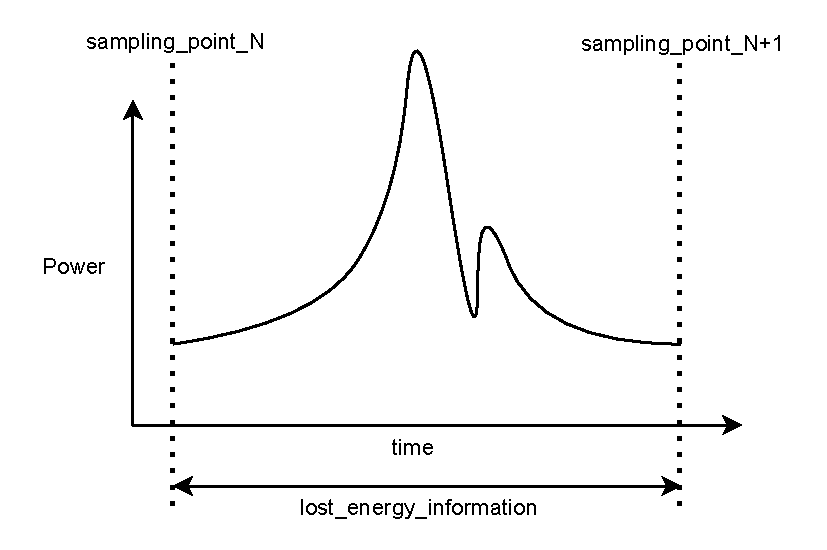
\includegraphics[width=0.7\textwidth]{assets/sampling_spike}
    \caption{
        Illustration of potential accuracy degradation connected
        to the limited power readings sampling/refresh rate.
    }
    \label{fig:sampling}
\end{figure}

The \cref{fig:sampling} aims to illustrate potential issues related to the
power reading refresh/sampling rate limitations. As can be seen the potential
short spike of power consumption between two sampling points will lead to
precision loss.

While this feature was not systematically explored in the present study, it
indicates a promising direction for future research. This topic will be
mentioned in later sections.

Second, it must be emphasized that the \texttt{ryzen\_smu} driver employed in
this work is not an official AMD release. Its functionality is largely the
result of community-driven reverse engineering efforts
\footcite{RyzenMonitor_GitHub,ryzen_managment_linux}. Consequently, exact
semantics of some registers and tables remain partially undocumented, which may
introduce uncertainties in the interpretation of results. Nevertheless, such
community tools represent the current state of the art for accessing low-level
telemetry on AMD platforms (predominantly for older architectures and desktop 
models) in the absence of official vendor support.

\subsection{Energy Measurement Framework}

\begin{figure}[htbp]
    \centering
    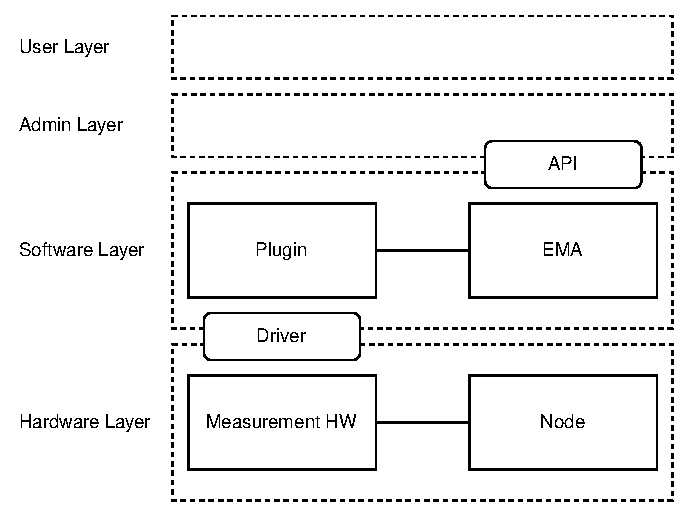
\includegraphics[width=0.7\textwidth]{assets/ema_arch}
    \caption{High-level architecture of \gls{EMA}.}
    \label{fig:ema_arch}
\end{figure}

For this study, the \gls{EMA} framework was selected as the primary tool
for collecting energy consumption data. The choice was motivated by several
key advantages:

\begin{itemize}
    \item \textbf{In-code integration:} \gls{EMA} allows precise measurement
          of energy consumption for specific regions (\cref{fig:ema_region})
          of application code, enabling multiple benchmarks to be integrated
          within a single code base.
    \item \textbf{Plug-in-based extensibility:} The framework supports multiple
          hardware measurement back-ends (e.g., \gls{RAPL}, Ryzen-specific
          sensors) concurrently through a uniform public interface, without
          modifying the application source.
    \item \textbf{Reliability:} \gls{EMA} handles common measurement
          pitfalls, such as counter overflows (\cref{fig:ema_rapl_overflow})
          in \gls{MSR}s, ensuring accurate and consistent data.
    \item \textbf{Familiarity and openness:} Author of this work has prior
          experience with \gls{EMA} and contributed to its development,
          facilitating integration and future tool improvements.
\end{itemize}

\begin{figure}[htbp]
    \centering
    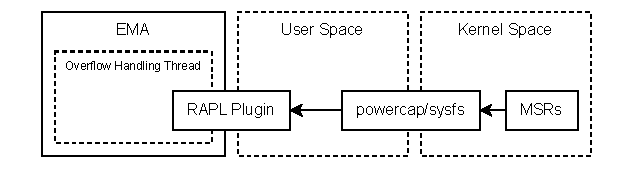
\includegraphics[width=0.7\textwidth]{assets/ema_rapl_overflow}
    \caption{Simplified illustration of overflow handling for \gls{EMA}'s \gls{RAPL} Plug-in.}
    \label{fig:ema_rapl_overflow}
\end{figure}

\gls{EMA}'s architecture is structured into layers, as illustrated in
\cref{fig:ema_arch}. The core of the framework is the \emph{Plug-in} system,
which encapsulates device-specific measurement logic while exposing a
consistent interface to the user. The \emph{User Layer} provides both
high-level and low-level \gls{API}s:
\begin{itemize}
    \item The high-level \gls{API} offers macros for defining measurement
        regions directly in code. 
    \item The low-level \gls{API} allows fine-grained control over plug-in
        management, region life-cycles, and data output.
\end{itemize}
\parencite{NAAICE}

\begin{figure}[htbp]
    \centering
    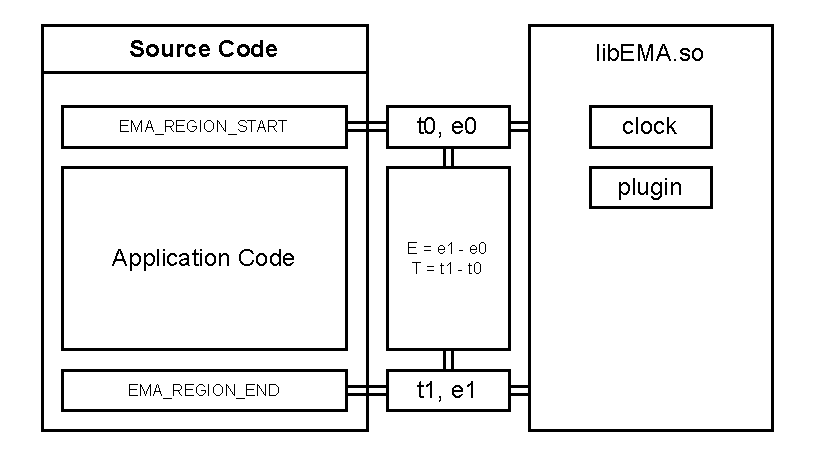
\includegraphics[width=0.7\textwidth]{assets/ema_region}
    \caption{Overview of \gls{EMA}'s Region API.}
    \label{fig:ema_region}
\end{figure}

These design choices make \gls{EMA} well-suited for integrating energy
measurements into experimental workloads and benchmarks, supporting
reproducibility and direct comparison across different measurement back-ends
\parencite{NAAICE}.

\subsection{Ryzen Plug-in}

To enable in-code energy measurements on AMD processors, a custom
\textit{Ryzen} plug-in was implemented for the \gls{EMA} framework.
\footnote{Source code available at
\url{https://github.com/SerhiiYahdzhyiev/EMA/tree/ryzen_plugin}.}

The plug-in uses the \texttt{libsmu} \footcite{RyzenSMU_GitHub} user-space
library to access the \gls{CPU}'s \gls{SMU} telemetry (\gls{PM} Table) and
selected \gls{SMN} registers. Readouts obtained
from the \gls{SMU} are exposed to \gls{EMA} as standard \emph{Device}
objects (structs) and thereby integrate with \gls{EMA}'s region-based
measurement model.

During initialization the plug-in queries the \gls{SMU} (via \texttt{libsmu})
to determine the platform codename and available telemetry fields. For
each logical measurement domain the plug-in creates a \texttt{Device}:
\begin{itemize}
  \item \emph{package} - total socket (socket / package) power;
  \item \emph{core} - aggregated power of all CPU cores;
  \item \emph{core.\(i\)} - per-core power measurements when available.
\end{itemize}
This device hierarchy enables reporting both coarse (socket) and finer
(per-core) energy estimates and matches \gls{EMA}'s device abstraction.

The plug-in samples instantaneous power values \(P\) (in watts) from the
\gls{PM} Table at time points \(t_k\). Energy is accumulated numerically
using a zero-order hold (rectangular) rule:
\[
  E(t_k) = E(t_{k-1}) + P(t_{k-1}) \cdot \Delta t,
\]
with \(\Delta t = t_k - t_{k-1}\)(\cref{lst:energy_uj}). In SI units this
yields energy in joules since
\(P\,[\mathrm{W}]\cdot\Delta t\,[\mathrm{s}] = E\,[\mathrm{J}]\).
In the implementation, internal counters is kept in micro-joules; hence,
when \(\Delta t\) is computed in microseconds the update reduces to:
\[
  E_{\mu\mathrm{J}} \mathrel{+}= P_{\mathrm{W}} \cdot \Delta t_{\mu\mathrm{s}}.
\]
The plug-in stores a per-device time-stamp to compute \(\Delta t\) and
exposes the accumulated micro-joules to the \gls{EMA}'s API.

\begin{samepage}
\begin{lstlisting}[
    language=c,
    caption={Energy accumulation in Ryzen Plug-in},
    label={lst:energy_uj},
    aboveskip=1.5\baselineskip,
    float
]
unsigned long long energy_uj = (unsigned long long)(power * delta_us);
d_data->energy_uj += energy_uj;
\end{lstlisting}
\end{samepage}

\paragraph{Practical considerations:}
\label{para:practical}
\begin{itemize}
  \item The integration method above corresponds to a rectangular
    approximation (\cref{lst:energy_uj}) (zero-order hold). It is simple and
    deterministic, but it can miss short high-power spikes if the sampling
    cadence is too low; this limitation is discussed above in the thesis.
  \item The plug-in uses dynamic mapping from the platform codename to
    \gls{SMN} offsets (table of known addresses), enabling reuse across
    several Ryzen codename variants.
  \item For \gls{RAPL}/\gls{MSR} measurements \gls{EMA}'s overflow handling
    utilities are applied to handle counter wraparound; for plug-in readings 
    though, the handling behavior is disabled due to lack of required values
    for the polling rate calculation.
\end{itemize}

On finalization the plug-in releases the \texttt{libsmu} context and
frees all per-device structures registered with \gls{EMA}.

This concise design allows simultaneous collection of \texttt{ryzen\_smu} and
\gls{RAPL} data within the same experimental run, which is required for the
comparative analysis described in this study.

\subsection{Benchmark Application and Automation}

To generate controlled \gls{CPU} workloads, a custom benchmark utility was
implemented \footcite{yahdzhyiev2025repo} (see source in
\path{code/src/bench.c}). The program was integrated directly with \gls{EMA}
to define multiple \emph{Measurement Regions} that emulate these distinct
workload patterns:

\begin{itemize}
  \item A short steady high computational load region.
  \item A long steady high computational load region.
  \item A short region with burst (spiked) computational load.
  \item A long region with burst (spiked) computational load.
  \item A short idle load region (sleep).
\end{itemize}

Between running each region a cooldown \texttt{sleep} call is made with
defined \texttt{COOLDOWN} time in seconds. For the main experiment run this
value was set to 5 seconds.

During each run the script \lstinline|run_measurements.sh|
(\cref{lst:run-measurements}) automates repeated executions and
programmatically switches the \gls{CPU} frequency-scaling governor to
\emph{performance} mode before taking all the measurements then switches it
back once completed). This ensures that energy measurements capture the
effect of dynamic frequency scaling policies on both \emph{burst} and
\emph{steady workloads}. Governor switching is achieved through the standard
\texttt{cpupower} interface provided by the Linux kernel.

For load generation, the benchmark uses a \texttt{stress-ng}
\parencite{stress-ng} to saturate the available CPU resources within each
measurement region. All measurements are collected via \gls{EMA}, enabling
simultaneous recording of \gls{RAPL}- and \gls{SMU}-based power data.

\subsection{Data Collection and Analysis}

To approximate the conditions of a \gls{HPC} cluster node, the target system
was placed in a minimal operating state during all measurement runs.
Non-essential services such as the graphical desktop environment, audio stack,
Bluetooth, and other user-oriented daemons were manually disabled.
Complete \texttt{systemd} service and process state dumps (one example
available in \cref{app:swspec}) were recorded before main experiment run to
document the exact runtime configuration. The corresponding dump files and the
shell script (\cref{lst:dump}) used to generate them are included in the
project repository \footcite{yahdzhyiev2025repo} for full reproducibility.

\begin{samepage}
\begin{lstlisting}[
    language=bash,
    caption={Script for \texttt{systemd state} dump},
    label={lst:dump},
    aboveskip=1.5\baselineskip,
    float
]
#!/bin/bash

set -e

systemctl list-units --all > baseline_units.txt
systemctl list-units --state=running > baseline_running.txt
systemctl list-unit-files --state=enabled > baseline_enabled.txt
systemctl list-sockets --all > baseline_sockets.txt
systemctl list-timers --all > baseline_timers.txt

ps -eo pid,ppid,cmd,%cpu --sort=%cpu > baseline-ps.txt
\end{lstlisting}
\end{samepage}

Raw energy-measurement outputs were subsequently processed using a set of
custom Python scripts. These scripts perform data filtering and validation,
visualization, and all statistical tests. The full preprocessing
(see \cref{tab:preprocessed} and \cref{lst:preprocess}) and analysis
tool-chain, together with instructions for use, is provided in the supporting
repository, referenced earlier, to allow independent reproduction of the
results.

\begin{table}[h]
\centering
\caption{Example of a preprocessed data layout}
\label{tab:preprocessed}
\begin{tabular}{llllrrr}
\hline
Plugin & Domain & Region & Energy (µJ) & Time (µs) & RunID \\
\hline
RAPL  & package & static\_10s & 726638158  & 10021131 & 13293 \\
RAPL  & core    & static\_10s &  92154704  & 10021145 & 13293 \\
RYZEN & package & static\_10s & 728919785  & 10021147 & 13293 \\
RYZEN & core    & static\_10s & 424903945  & 10021321 & 13293 \\
RAPL  & package & idle\_10s   & 142281003  & 10001493 & 13293 \\
RAPL  & core    & idle\_10s   &     35277  & 10001517 & 13293 \\
RYZEN & package & idle\_10s   & 143887347  & 10001517 & 13293 \\
RYZEN & core    & idle\_10s   &         0  & 10001677 & 13293 \\
RAPL  & package & static\_60s & 4151276239 & 60020666 & 13293 \\
RAPL  & core    & static\_60s &  506078183 & 60020675 & 13293 \\
RYZEN & package & static\_60s & 3827742587 & 60020678 & 13293 \\
RYZEN & core    & static\_60s & 2424841798 & 60020840 & 13293 \\
RAPL  & package & burst\_10s  & 455822711  & 10101399 & 13293 \\
RAPL  & core    & burst\_10s  &  44832536  & 10101350 & 13293 \\
RYZEN & package & burst\_10s  & 157008581  & 10101348 & 13293 \\
RYZEN & core    & burst\_10s  &    444245  & 10101359 & 13293 \\
RAPL  & package & burst\_60s  & 2626776556 & 60129708 & 13293 \\
RAPL  & core    & burst\_60s  &  265875563 & 60129730 & 13293 \\
RYZEN & package & burst\_60s  &  901179043 & 60129732 & 13293 \\
RYZEN & core    & burst\_60s  &         0  & 60129978 & 13293 \\
\hline
\end{tabular}
\end{table}

For development and debugging of the data-processing pipeline, an initial
trial run with a reduced number of benchmark iterations \footnote{Five, to be
precise.} was performed. This smaller dataset enabled rapid refinement of
the scripts before the full-scale experiments.

Both the trial and main data are provided in a raw format in the supporting
repository, accompanied by a detailed \texttt{README} that explains how to
reproduce analysis and visualization used in this work.
